\documentclass{article}
\usepackage{enumitem}
\usepackage{fancyhdr}
\usepackage{listings}
\usepackage{graphicx}
\usepackage{wrapfig}
\usepackage{hyperref}
\usepackage{supertabular}
\usepackage[lastexercise,answerdelayed]{exercise}
\usepackage[table]{xcolor}
\usepackage{todonotes}
\usepackage{multicol}

% for exercise 
%% Change this for title information 
\pagenumbering{roman}
\newcommand\ExTitle{\ Course Outline and Essential Information}
\author{Siobh\'an Roche, Mair\'ead Meagher, S.E.T.U.}

\newcommand\fullExTitle{Programming Fundamentals 1 \\Semester 1 - 2025-2026}
\newcommand\footerExTitle{\ExTitle -\ Programming Fundamentals 1}

\pagestyle{fancy}
\fancyhead{} % clear all header fields
\renewcommand{\headrulewidth}{0pt} % no line in header area
\fancyfoot{} % clear all footer fields
\fancyfoot[LE,RO]{\thepage}           % page number in "outer" position of footer line
\fancyfoot[RE,LO]{\footerExTitle} % other info in "inner" position of footer line

%\usepackage[mathrm,colour,cntbysection]{czt}

\begin{document}
\begin{Huge}
	\begin{center}
	\fullExTitle \\
    \vspace{1cm}
    Course Outline and Essential Information
    \vspace{.1cm}
    \end{center}
\end{Huge}
\vspace{1.5cm}
\begin{center}
    \begin{tabular}{|c |  c | }
    \hline
    \multicolumn{2}{|c|}{Module Lecturers} \\
    \hline
    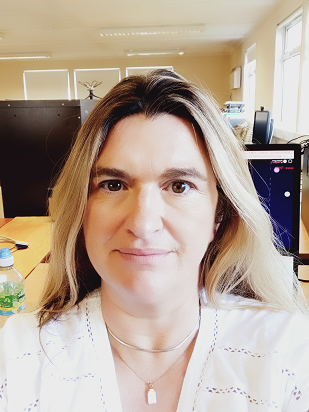
\includegraphics[width=1.5in]{img/siobhan3.png} &          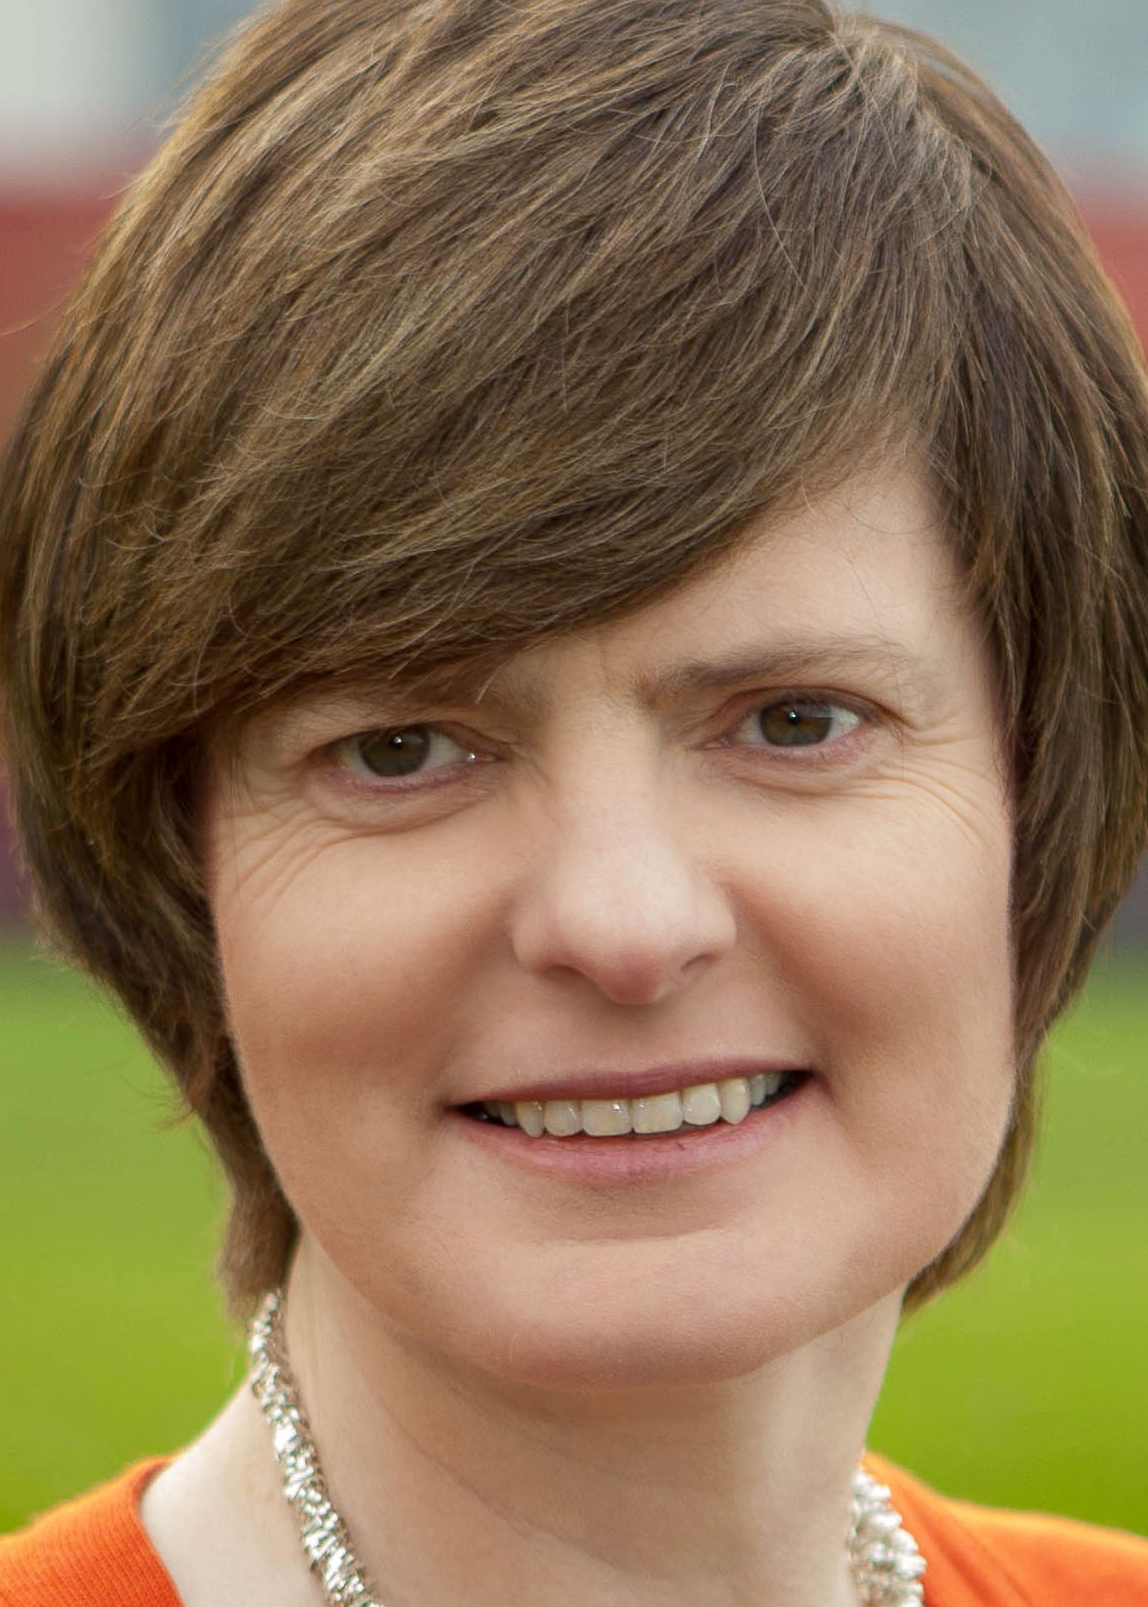
\includegraphics[width=1.5in]{img/mairead.png} \\ 

       Dr Siobh\'an Roche, & Mair\'ead Meagher  \\  
       \href{mailto:siobhan.roche@setu.ie}{siobhan.roche@setu.ie} & \href{mailto:mairead.meagher@setu.ie}{mairead.meagher@setu.ie} \\
  
    \hline
    \multicolumn{2}{|c|}{Department of Computing and Mathematics} \\
     \hline

  
    \end{tabular}
\end{center}

\vspace{-.5cm}
    \begin{figure}[h]
    
        \centering
        
\includegraphics[width=3in]{img/RGB.png}
    \end{figure}
\thispagestyle{empty} 
\pagebreak
\tableofcontents
\thispagestyle{empty} 
\pagebreak
\pagenumbering{arabic}
\section{Module Name}   
Programming  Fundamentals 1 \\
\section{Lecturers}
Siobh\'an Roche, \href{mailto:siobhan.roche@setu.ie}{siobhan.roche@setu.ie}, 
Lecturer in Department of Computing and Mathematics.\\
Siobh\`an will take lectures and labs for groups W3 and W4 in this module.\\
Mair\'ead Meagher, \href{mailto:mairead.meagher@setu.ie}{mairead.meagher@setu.ie}, 
Lecturer in Department of Computing and Mathematics.\\
Mair\'ead will take lectures and labs for groups W1 and W2 in this module.\\
\section{How to reach us}
\begin{itemize}
    \item The quickest way to reach us  is via Slack. 
    Please join the Programming Fundamentals 1 Slack workspace 
    \ \href{https://join.slack.com/t/progfund2025-2026/shared_invite/zt-37df9qgwi-gNEmD0q15QMT53DHASESLQ}{here}. 
    We  will be using this a main form of 'outside class' communication for this module. 
    If you have a general query, please use the \textbf{\#general} channel. 
    If you need to contact us directly, please DM one or both of us rather than using public channels. 
    You should  normally contact the lecturer that you see face-to-face about most matters 
    (i.e. either Maire\'ad or Siobh\'an) but feel free to copy us both. 
    \item You can also reach us  via email:
    \begin{itemize}
        \item \href{mailto:siobhan.roche@setu.ie}{siobhan.roche@setu.ie}   
    and\textbackslash{}or \item \href{mailto:mairead.meagher@setu.ie}{mairead.meagher@setu.ie}. 
\end{itemize} We are available during work hours from Monday to Friday, 9am to 5pm. 

    You can email/Slack us outside of these hours and we will reply as soon as we can, 
but always within three days.(If this does not happen, assume your contact has gone into spam etc. 
and please re-contact us.) When emailing us, please indicate what module you are taking as well as 
the nature of your query in the subject line, and do not forget to use an appropriate greeting and sign off. 
It’s important to be polite and to treat one another with 
respect; let’s start as we mean to go on.
   
\end{itemize}
\pagebreak
\section{Learning Technologies}
\begin{itemize}
\item All lectures and labs  will happen in person as per timetable.
\item We use tutors to publish the material for this  module. This static website will hold all the notes, labs and links to videos.  See Figure \ref{tutors}.
This site is organised by topic,as opposed to Moodle which is organised by week(by linking to, among other things,  the relevant tutors topic).
\begin{figure}[h]
\centering
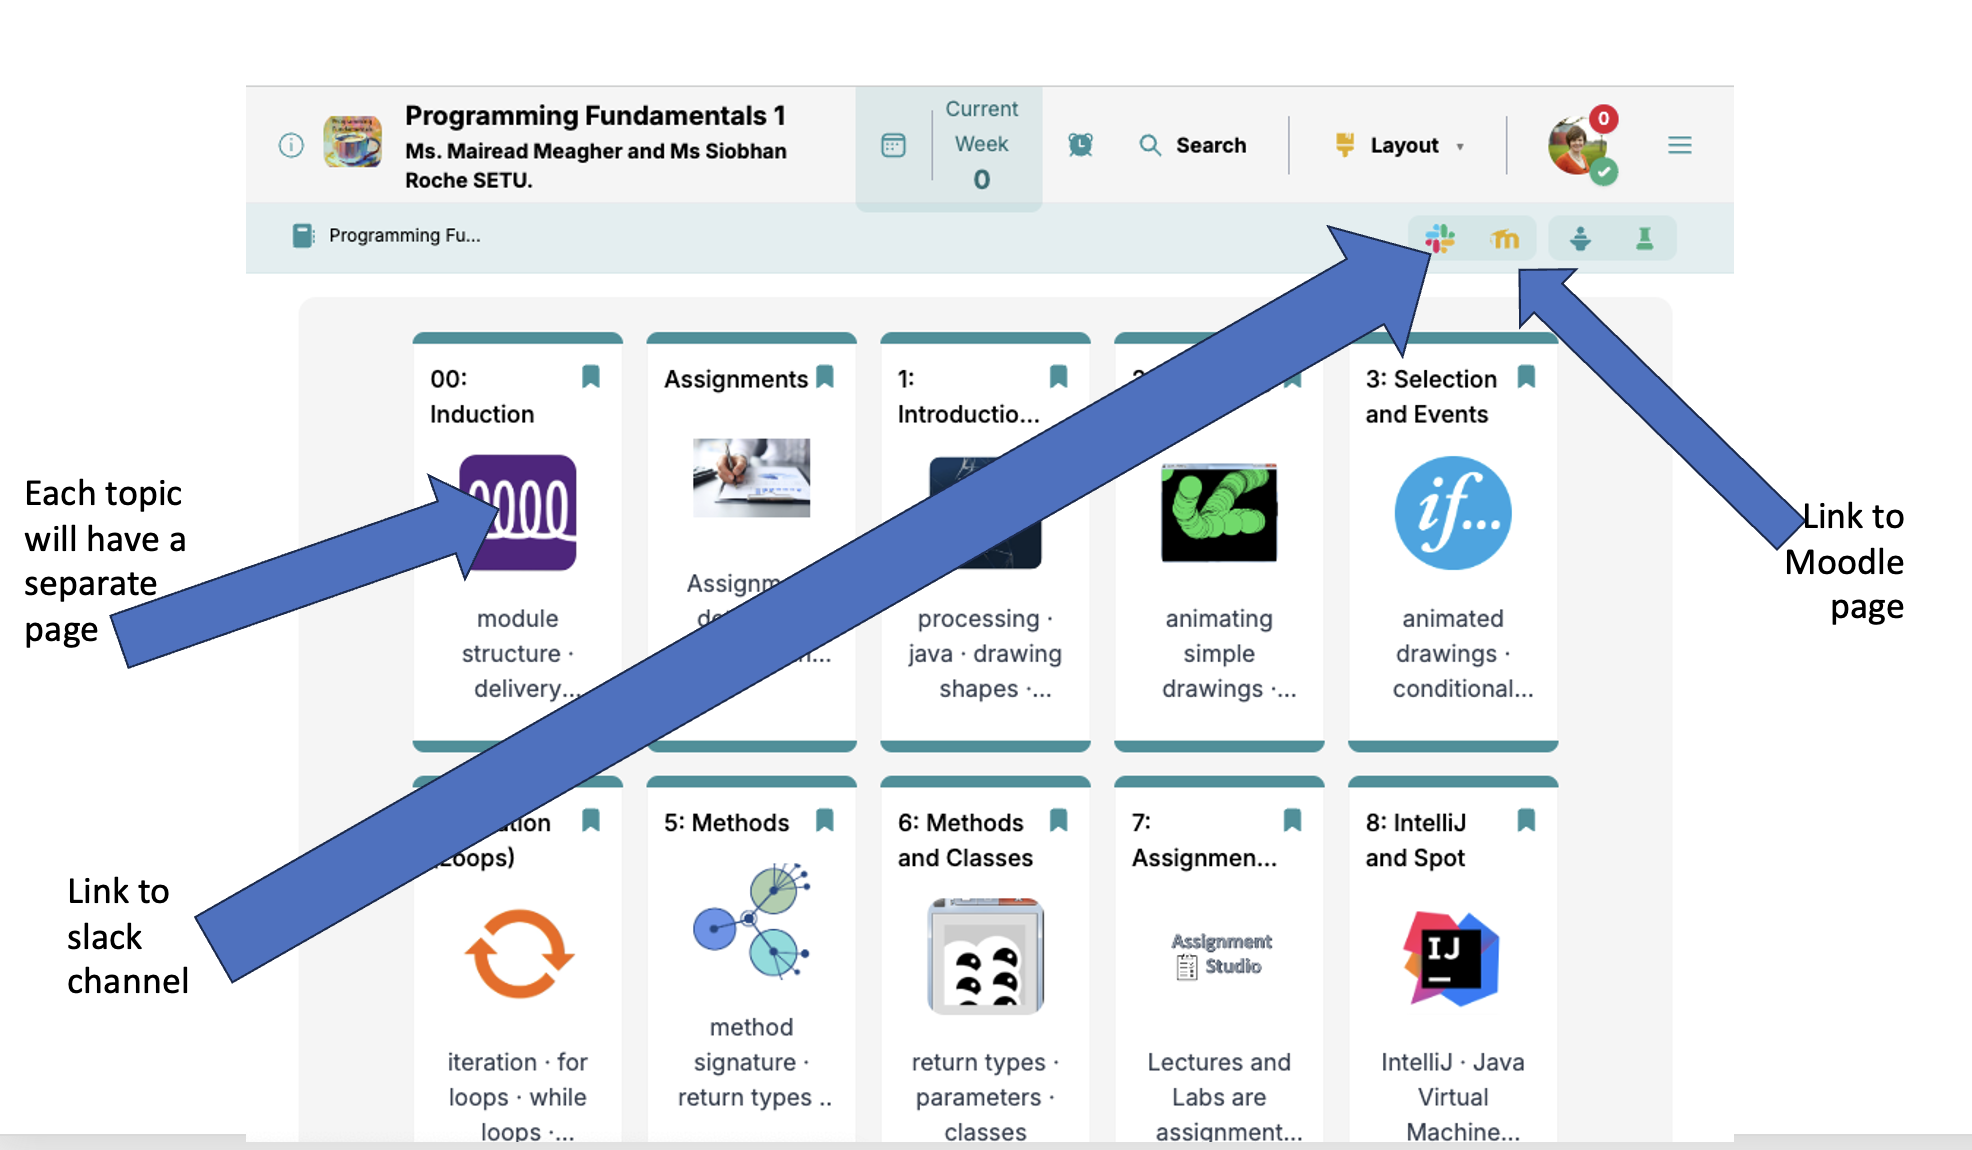
\includegraphics[width=.6\textwidth]{img/proc-tutors.png}
\caption{Example of tutors website}
\label{tutors}
\end{figure}

There are a number of visual themes available across the site.  See Figure \ref{visual}.
Of particular note, there is a font which is dyslexia-friendly. This is marked on the diagram. 
\begin{figure}[h]
\centering
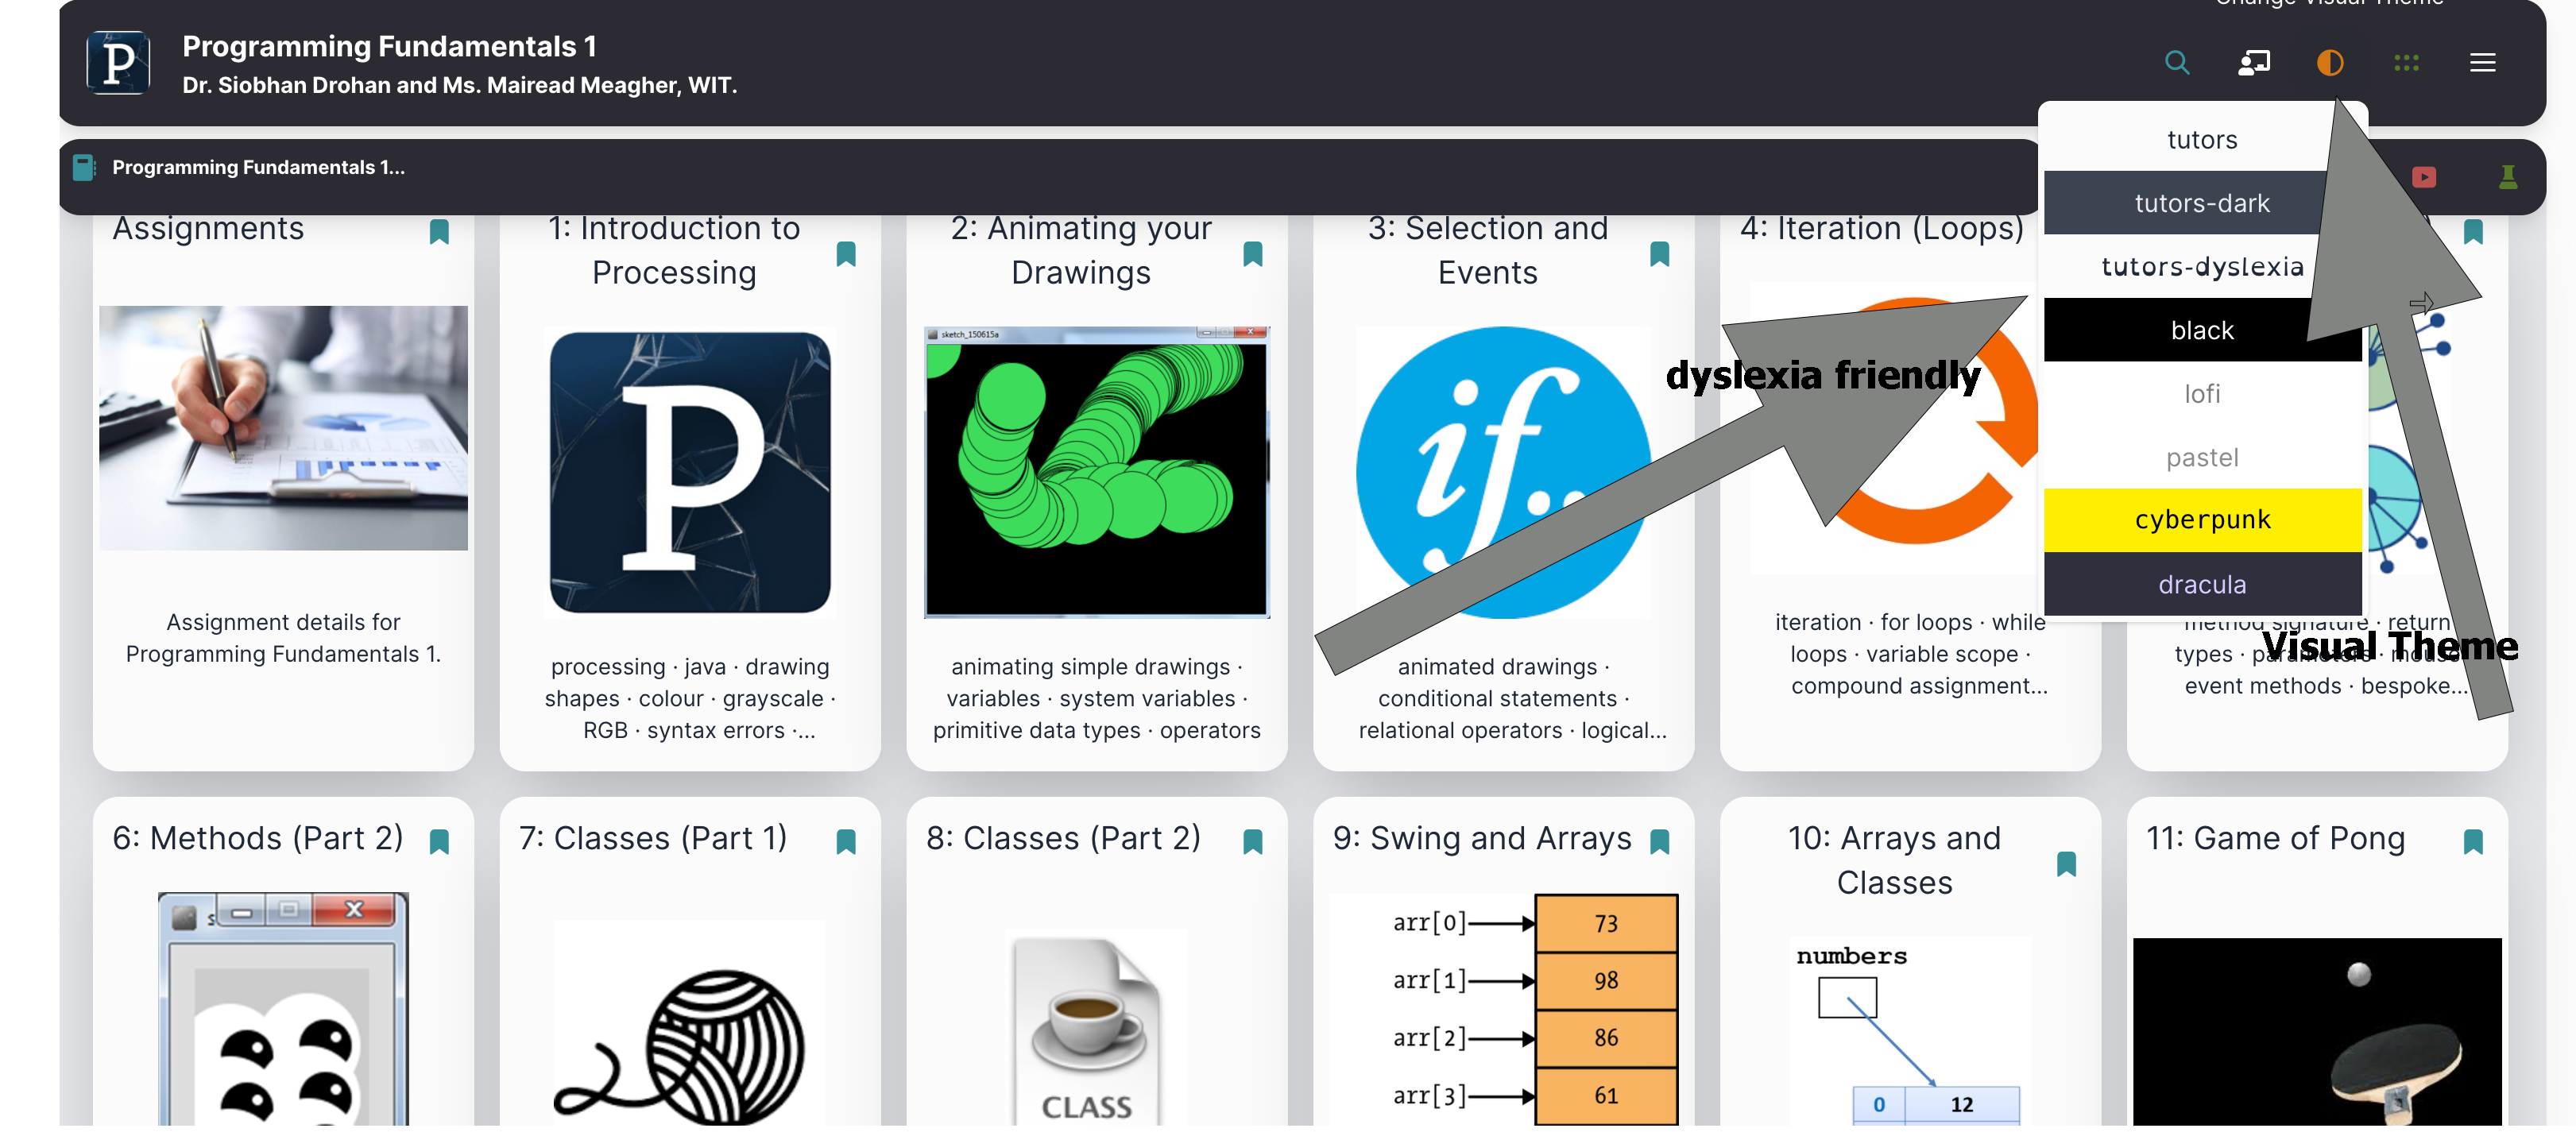
\includegraphics[width=.6\textwidth]{img/v-theme.png}
\caption{Visual themes in tutors}
\label{visual}
\end{figure}
\item \textbf{Moodle} - our learning management system(used all over SETU, Waterford campus), 
where you can find links to the notes, and where online exams are curated. The link to this course is \todo{put in Moodle link}{here}.  
Each week you will be given a list of activities to have done before the class and 
a list of activities to have done before the next week. 
The link to the Moodle page for this module is 
\todo{insert Moodle link} {here}.  \\
Each week there will be a set of links made available to you for that week including: 
\begin{itemize}
    \item Links to topics in the tutors website (see below)
    \item Links to 'dropboxes' for the labs for that week (see below)

\end{itemize}


\item \textbf{Slack} - our main form of communication outside of 
class. See above for links.

\item \textbf{GitHub} - we will be using GitHub for the tutors website.   
\textbf{To use tutors, you will need to have a GitHub account. (https://github.com/) For the moment this is not necessary but we will turn this system on in Week 3.} 

\end{itemize}

\pagebreak
\section{Module objectives /\ Learning outcomes and schedule of teaching}

\subsection{Module objectives and Learning Outcomes}

On completion of this module students should be able to: 
\begin{enumerate}
   \item Apply core problem solving approaches suitable to the programming discipline to build algorithms.
   \item Write small applications using standard sequence, conditional and iterative control structures.
   \item Modify and expand small applications.
   \item Write small applications that use simple UI, computation and data structures.
   \item Develop techniques to effectively test, debug and document small applications.
   \item Analyse and explain how the above applications work.
   \item Write a simple object-oriented program using the \textit{BlueJ} environment.
\end{enumerate}

\textbf{ \textit{Note:}} We do not expect you to have \textbf{any} prior experience of programming, either in Java or any other language. 
We will start from the very beginning and build up from there.

For this module, we will be using Java, and using the \textbf{\textit{blueJ}}\footnote{https://www.bluej.org/} environment. 


Note that note that \textbf{\textit{blueJ}}
is available free to use. Details of how to download it will be in the labs before we use them. 
\pagebreak 

\subsection{Schedule of Teaching}
The schedule of teaching is given in Table \ref{schedule}. 
 Week 1 will start on Monday 15th September.
\begin{figure}[h]
    \centering
    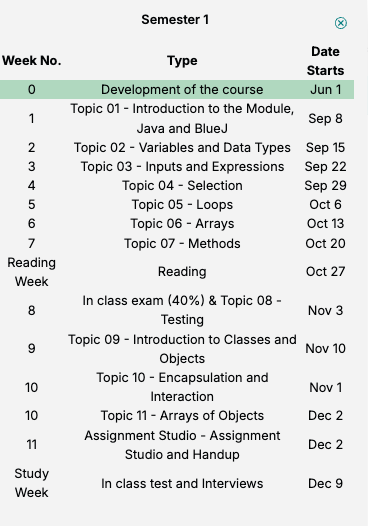
\includegraphics[width=.6\textwidth]{img/schedule.png}
    \caption{Week-by-week schedule of teaching}
    \label{schedule}
    \end{figure}
This may change slightly as the semester progresses.

This list of weekly topics is also available on the tutors page for this module - top row.
  \pagebreak
\section{Assessment Breakdown} 
The assessment in this module is \textbf{100\%} Continuous Assessment made up of three components. There will be no final examination in this module. 
\subsection{Continuous Assessment (100\%) }
Your module assessment  is made up of:  
    \begin{itemize}
        \item \textbf{Attendance at tutorials (10) - 10\%.} You are  asked to attend your tutorials where written problem sheets will be given and so that you can practice any new concepts. 
        \item \textbf{Written in class test - 40\%.} This will be a test based on the material covered in the first half of the module and largely based on tutorial sheets and labs. 
        \item \textbf{Programming Assignment  - 50\%. }
        Having practiced the material in the first half of the module, you will be asked to complete a programming assignment which uses the material covered in the first half of the module and the new material covered in the second half of the module.
        
        You will be asked to solve a problem using classes, methods and arrays. The problem will be fully specified and you will be asked to implement it in \textbf{\textit{Java}} using the \textit{blueJ} environment
    \end{itemize}

  \begin{table}
    \begin{center}
        \begin{tabular}{|c|c|c|c|}
            \hline
            \rowcolor{red!60}
            \textbf{Assessment} & In-class & Programming & Tutorial  \\
               \rowcolor{red!60}
            \ & Test & Assignment &  attendance \\

            \hline
            \rowcolor{red!30}
            \textbf{Week No.} & Week 8 & Week 12 & each Week \\
            \hline
            \rowcolor{red!30}
            \textbf{Time of test/} & During  & 18:00,  & n/a \\
            \rowcolor{red!30}
            \textbf{Time /Deadline} & class time& Sunday 7th Dec.& \\
            \hline
            \rowcolor{red!35}
            \textbf{Written exam} & none & Monday 8th Dec. & n/a \\
            \hline
            \rowcolor{red!40}
            \textbf{Interview} & n/a & Week 12/13 & n/a \\
            \hline
            \rowcolor{red!60}
            \textbf{Percentage} & 40\% & 50\% & 10\% \\
            \hline
        \end{tabular}
        \caption{Assignment Schedule}
        \label{tab:ass-schedule}
    \end{center}
\end{table}





In the case of the in-class test, you will get your marks back as soon as is possible, but usually within a week. 
If you are wondering why you got a particular mark, \textbf{always} ask us. Our marking schemes are very comprehensive and 
we are happy to go through the breakdowns with you. 
We don't give this comprehensive feedback by default to speed up the return of the marks, but are happy to engage with you  about them later. 

In the case of the programming  assignment, the marks are not published as the final mark is overseen by the external examiner and the 
finalised mark is released only after the examinations are fully processed.
to sit an in-class test based around your assignment. This is to help us during our interview process for this assignment. 
However, we will be happy to go through those marks with you 
after the results have been processed and finalised. 

Also, in the case of this programming assignment, you will be asked 
to sit an in-class test based around your assignment. This is to help us during our interview process for this assignment. 
Please take this opportunity to clarify any queries you have. This is a good way to ensure that 
you are attempting the work in a suitable manner.


For the programming assignments, a \textbf{marking scheme will be published with the specification of the assignment}. Be sure that you are aware of the marking scheme. 
If there are marks going for a particular part, and you haven't attempted that part, we cannot give you any marks for that part! . 
\begin{quote}
 \textbf{\textit{Always make it easy for the examiner to give you marks.}}
\end{quote}

If you wish to seek an extension for an assignment, you must do so in sufficient time (i.e. not on the day of submission, and not 
when the submission date has passed) and must provide a valid reason for seeking the extension. 


\section{Academic Integrity}
The School of Science and Computing  at South Eastern Technological University (Waterford) are  committed to maintaining the highest standards of academic integrity. 
Academic misconduct, including, but not limited to, 
cheating may result in a mark of zero for the assignment as well as disciplinary action.
 Additional sanctions may by imposed depending on the case. 


 You are responsible for ensuring that you do not get involved in cheating of any kind. This includes non-referenced code, 
 AI generated code, copying code from the internet, copying code from another student,
    allowing another student to copy your code, etc..
 
 With regard to programming submissions, \textbf{an interview is mandatory and is part of your assignment mark (as a multiplier)}. 
 The interview is to ascertain that the work is your own and that you fully understand how it works, in its elemental parts and how it works together. 
 
We  will always encourage you to work in collaboration with your fellow classmates. But please be careful not to cross the line between collaboration and using someone else's work. 
 Please do not be tempted to use this route. 
 It is too risky and the penalty can affect your academic future. 
\pagebreak
\section{Engagement in the module and Time Management}
\subsection{Engagement}
 Part of active engagement  for any module involves a degree of time management. 
 As part of this module we will be asking you to complete exercises, between class times. 
 Each week, for instance you will be asked to complete labs (available on Moodle) and upload your attempt on Moodle.
 These will not be graded but, by engaging in these tasks at the time, you will be in a better position to 
 understand the next part of the module and to attempt the assignments. We will approach the module in a step-by-step manner, 
 so opting out at any part will make it more difficult for you to keep up. 
 This is where time management will come in - you need to be careful to ensure that you keep a balance between modules. 
 
 Always ask questions, either in class or during labs.  One way to help to stay engaged is to ask questions if you don't understand what is going on. 
 Remember, when you are asking questions:
 \begin{enumerate}
    \item Just the process of asking a question means that you have learned something. 
    \item If you cannot understand, in most cases, you are not the only one. 
    \item Asking questions means that the pace of the lecture/ labs will suit you better - we will always keep going if there are no questions! 
 \end{enumerate}
 \subsection{Time Management}
 There are many software tools available to help you managing yout time and in general helping you to plan your work. Have a look around - see if any of them suit you. You should \textbf{not} have to pay for one there are plenty Open Source versions and in some cases there are free educational versions (always check this out)
 A couple that are worth mentioning: 
 \begin{itemize}
     \item \href{https://trello.com/en}{\textbf{Trello}} - this is  great Project Management Tool - it's Open Source and used in the software industry
     \item \href{https://www.notion.so/}{\textbf{Notion}} is a commercial product but free to students - you just need to register. There are many templates available for your use - it's well worth a look. 
     \item A notebook! 
 \end{itemize}
 Learning how to organise your material/ thoughts / ideas is a very good use of your time. It may be one of the most valuable things you learn. 
 
 \section{Organizing yourself}
 \subsection{Organisation of your labtop/cloud storage}

\begin{wrapfigure}{r}{0.25\textwidth} %this figure will be at the right
    \centering
    
\includegraphics[width=0.2\textwidth]{img/chaos.jpg}
\end{wrapfigure}

It is really important to organise where you store all your college files/ software.
If you don’t do this early, chaos will ensue! The best way is to organise your files from the start. 
You can use this file structure on Cloud (One-Drive?) and mirror it on your labtop so you can 'backup' easily by dragging the full folder from one to the other. 
If you are using a labtop, then you can use your local drive but be sure to back it up regularly.
  
\subsection{Suggested Filing System}

A suggested filing system is given in Fig \ref{filing}. Note you could have subfolders named Week 1 etc. whichever is most appropriate. 

Having set this up, you will get used to using this very quickly and you will save a lot of time in the long run. 
\begin{figure}[h]
\centering
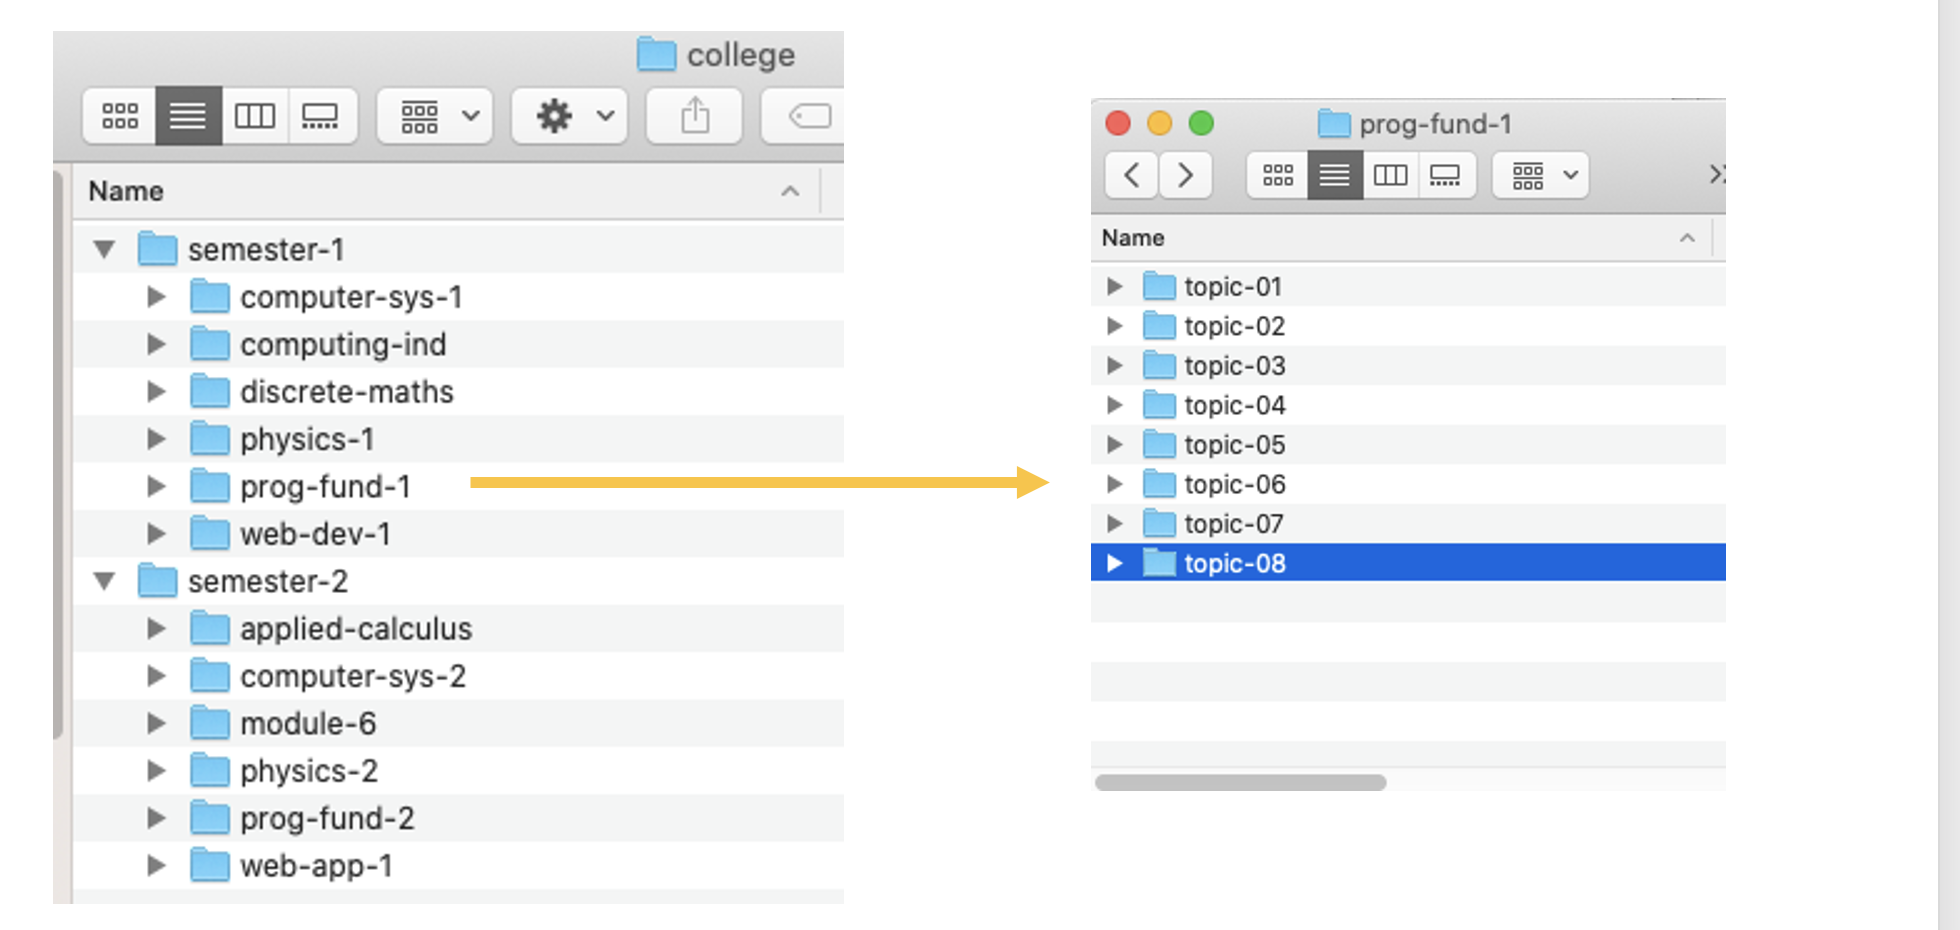
\includegraphics[width=.6\textwidth]{img/filing.png}
\caption{Suggested Filing System}
\label{filing}
\end{figure}
\newcolumntype{a}{>{\columncolor{green}}c}
\newcolumntype{b}{>{\columncolor{red}}c}
\colorlet{shade1}{green!80!red}
\colorlet{shade2}{green!70!red}
\colorlet{shade3}{red!90!red}
\colorlet{shade4}{red!80!red}
\colorlet{shade5}{yellow!20!red}

\begin{table}[h]
\begin{center}
    \begin{tabular}{ | m{15em}   |m{15em}  }    
        %  \begin{tabular}{ |>{\columncolor[gray]{0.8}} m{10em} |b m{10em}|  } 
        \hline
    \rowcolor{shade3}
    \cellcolor{shade1}DO's & DON'T's   \\ 
     \hline  
     \rowcolor{shade4}
     \cellcolor{shade2} Set up the folder structure and continue to use it. 
     & Set up and use it ‘an odd time’.
     \\  
     \rowcolor{shade4}
     \hline
     \cellcolor{shade2}Set up ‘favourites’ folder in Explorer/Finder for your ‘college’ subfolder
 & Use Downloads or Desktop as the root folder for ‘college' subfolder. \\ 
 \hline
     \rowcolor{shade4}
     \cellcolor{shade2}Store data (weekly homework, etc.) using this structure.
     &Mix up data and programs in college folder.
     \\ 
     \hline
     \rowcolor{shade4}
     \cellcolor{shade2}Store your software (e.g. BlueJ) in another folder e.g. /dev or Program Files.
 &   \\ 
     \hline
 
  
    \end{tabular}
    \caption{Do's and Don't's of Filing Systems}
    \label{tab:dos-donts}
\end{center}
\end{table}

\vspace{2cm}
\begin{figure}[h]
    \centering
    
\includegraphics[width=.8\textwidth]{img/good-luck.jpeg}

    \end{figure}

Finally, we wish you all the best of luck with this module and all of your university experience,
\vspace{1cm}

Siobh\'an and Mair\'ead.

\end{document}